%%%%%%%%%%%%%%%%%%%%%%%%%%%%%%%%%%%%%%
% 1. Presentation header file (in separate file)
%%%%%%%%%%%%%%%%%%%%%%%%%%%%%%%%%%%%%%
\documentclass[pdf]{beamer}
%\input{texfile} % replace texfile with main content file name

%%%%%%%%%%%%%%%%%%%%%%%%%%%%%%%%%%%%%%
% 2. Handout header file (in separate file)
%%%%%%%%%%%%%%%%%%%%%%%%%%%%%%%%%%%%%%
%\documentclass[handout, t]{beamer}
%\input{texfile} % replace texfile with main content file name




%%%%%%%%%%%%%%%%%%%%%%%%%%%%%%%%%%%%%%
% 3. Main content preamble and opening slides
%%%%%%%%%%%%%%%%%%%%%%%%%%%%%%%%%%%%%%
%\mode<beamer>{
%\usetheme{Frankfurt}
%\setbeamertemplate{navigation symbols}{}
%}
%<hadout>
\mode<presentation>{
\usepackage{pgfpages}
\usepackage{graphicx}
\usepackage{tikz}
%\pgfpagesuselayout{4 on 1}[a4paper, border shrink=10mm, landscape]
\usetheme{default}
}
\usepackage{beamerthemesplit}
\title{Wireless Networks }
\subtitle{CS 3251}
\author[Abhinav Narain]{Abhinav Narain \\
 slides content from Alex Snoeren,Professor, UCSD  }

\institute{Georgia Institute of Technology}
\date{}

\begin{document}
\mode*
\begin{frame}
  \titlepage
\end{frame}

\begin{frame}
  \frametitle{Outline}
  \tableofcontents
\end{frame} 

\begin{frame}{Modes in 802.11}
  \begin{itemize}
   \item Infrastructure mode 
   \item Ad-hoc mode
\end{itemize}
   \begin{center}
       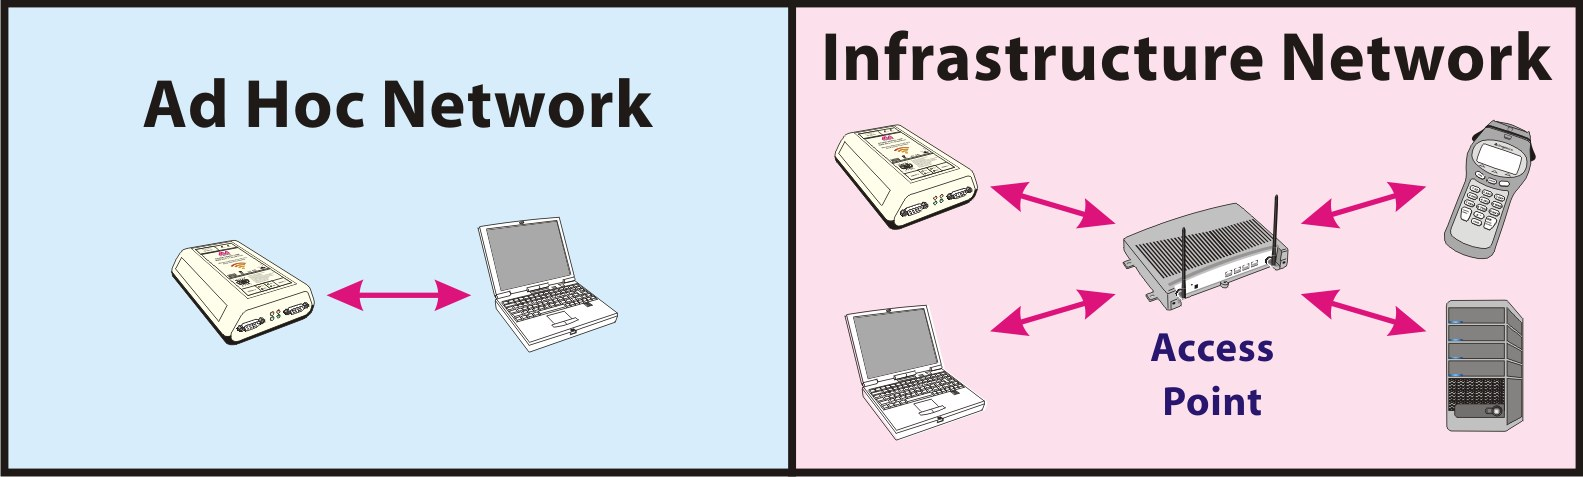
\includegraphics{ad_hoc__infrastructure.jpg}%[width=11cm]  
   \end{center}
\end{frame} 

\begin{frame}{Infrastructure mode}
  \begin{itemize}
  \item Fixed terminal (lets say www.google.com), sends an ethernet frame
  \item The mac header of the ethernet frame(with 802.3 ethernet header) is transformed into a $802.11$ mac header on your wireless router and transmitted on the wireless medium using $802.11$ PHYsical layer
  \end{itemize}
   \begin{center}
       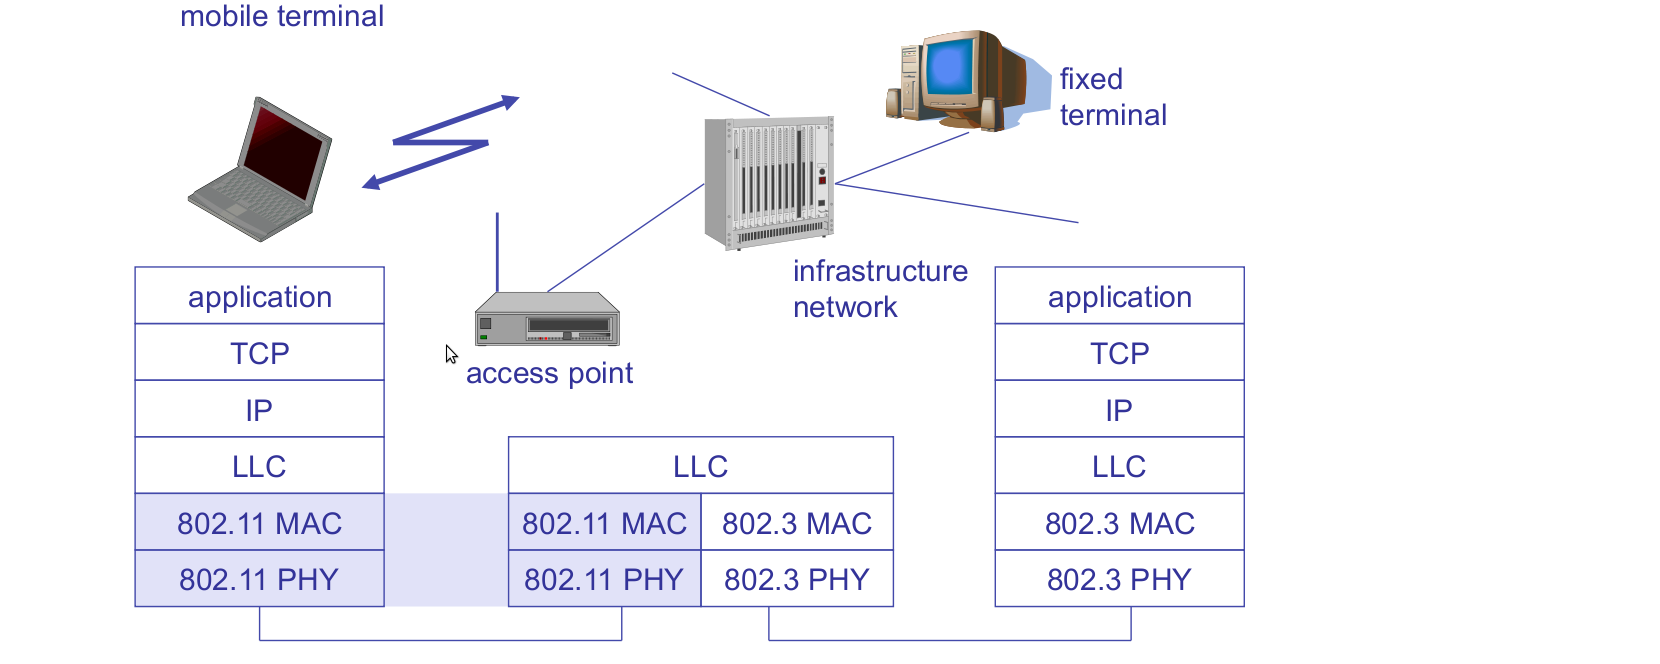
\includegraphics[scale=.2]{infra.png}%[width=11cm]  
   \end{center}
\end{frame} 

\begin{frame}{802.11 Layers and functions}
  \begin{columns}
    \begin{column}{.5\textwidth}
      \begin{itemize}
      \item MAC
        \begin{itemize}
        \item access mechanisms, fragmentation, error control, encryption 
        \end{itemize}
      \item MAC Management         
        \begin{itemize}                                                                                                                         
        \item synchronization, roaming, MIB, power management                       
        \end{itemize} 
      \end{itemize}
    \end{column}
    \begin{column}{.5\textwidth}      
      \begin{itemize}
      \item PLCP Physical Layer Convergence Protocol(carrier sense)
        \begin{itemize}
        \item clear channel assessment signal
        \end{itemize}
      \item PMD Physical Medium Dependent
        \begin{itemize}
        \item modulation, coding
        \end{itemize}
      \item PHY Management
        \begin{itemize}
        \item channel selection, MIB                                      
        \end{itemize}
      \item Station Management
        \begin{itemize}
        \item coordination of all management functions
        \end{itemize}
      \end{itemize}
    \end{column}
  \end{columns}
\end{frame}

\begin{frame}{802.11 Physical Layers}
  \begin{itemize}
  \item 802.11b - 2.4 GHz ISM band
    \begin{itemize}
    \item  FHSS (Frequency hopping spread spectrum); deprecated
    \item  DSSS (Direct sequence spread spectrum)
    \item  Up to 11 Mbps
    \item  300m outdoor, 30m indoor 
    \end{itemize}     
  \item   802.11a/g - 2.4 GHz ISM band / 5.0 GHz UNII band
    \begin{itemize}
    \item  OFDM (Orthogonal frequency domain multiplexing)
    \item  Up to 54 Mbps
    \end{itemize}
  \item   802.11n - 2.4/5.0 GHz bands
    \begin{itemize}
    \item  Adds MIMO and other tricks to 802.11g     
    \item  Up to 300-500 Mbps!
    \end{itemize}    
  \item Each backwards compatible with the previous ones
  \end{itemize}
\end{frame}
%slide 

\begin{frame}{802.11b Physical Channels}
  \begin{itemize}
  \item   12 channels available for use in the US
    \begin{itemize}
    \item  Each channel is $20+2$ MHz wide
    \item  Only 3 orthogonal channels
    \item  Using any others causes interference           %image needed for ortho bands
    \end{itemize}
  \end{itemize}
\end{frame}

%slide 
% Motivation for multicarrier modulation
\begin{frame}{ Multipath Interference}
  \begin{itemize}
  \item   RF signals bounce off of objects (e.g., walls)
    \begin{itemize}
    \item  Reflected  signals travel different distances to receiver
    \item  Difference in distance leads to difference in delay
    \end{itemize}
  \item   Limits effective modulation rate in 802.11b  AirTight Networks
  \end{itemize}
\end{frame}

%slide 

\begin{frame}{Avoiding ISI: OFDM }   
  \begin{itemize}
  \item  Break data up into multiple separate streams
    \begin{itemize}
    \item  Transmit each stream independently on different frequency
    \item Pack frequencies
    \end{itemize}
  \end{itemize}
  %image needed
\end{frame}

%slide 
\begin{frame}{ 802.11a/g/n ODFM PHY}
  \begin{itemize}
  \item Each 20-MHz channel
    \begin{itemize}
    \item Subcarriers spaced appropriately, 4 used as ``pilots''
    \end{itemize}
  \end{itemize}
\end{frame}

%slide 

\begin{frame}{802.11n: MIMO}
  \begin{itemize}
  \item   Use multiple physical antennae simultaneously
    \begin{itemize}
    \item Spatial multiplexing: split data cross antennae
    \item Space-Time Block Coding: same data, encoded differently
    \item Transmit beamforming: steer the signal toward the receiver 
    \end{itemize}
  \end{itemize}
\end{frame}

%slide 

\begin{frame}{Carrier Sense Multiple Access}
\textcolor{red}{CSMA}: listen before transmit
  \begin{itemize}
  \item If channel sensed idle: transmit entire packet
  \item If channel sensed busy, defer transmission
    \begin{itemize}
    \item Persistent CSMA: retry immediately with probability p when channel becomes idle (may cause instability)
    \item Non-persistent CSMA: retry after random interval
    \end{itemize}
  \item But what about collisions?
  \end{itemize}
\end{frame}
%slide 

\begin{frame}{CSMA/CA}
  \begin{itemize}
  \item Impossible to hear collision w/half-duplex radio
  \item Wireless MAC protocols often use \textcolor{red}{collision avoidance}
    techniques, in conjunction with a \textcolor{red}{(physical or virtual) carrier
    sense} mechanism    
  \item Collision avoidance
    \begin{itemize}
    \item  Nodes negotiate to reserve the channel.     
    \item  Once channel becomes idle, the node waits for a randomly chosen
      duration before attempting to transmit
    \end{itemize}
  \end{itemize}
\end{frame}

%slide
\begin{frame}{Challenge Reliability}
  \begin{itemize}
  \item Wireless links are prone to errors. High packet loss rate detrimental to transport-layer performance.
  \item Mechanisms needed to reduce packet loss rate experienced by upper layers
  \end{itemize}
\end{frame}

\begin{frame}{Link-layer ARQ}
  \begin{itemize}
  \item When B receives a data packet from A, B sends an Acknowledgement (ACK) to A.
  \item If node A fails to receive an ACK, it will retransmit the packet
  \end{itemize}

  \begin{figure}
    \begin{center}
      \begin{tikzpicture}
        % draw nodes (pgf/TikZ v2.00 manual sections 3.4, 3.7, 3.9)
        \node (Client) at (0,0) [circle,draw,label=below:A] {$A$};
        \node (Receiver) at (3,0) [circle,draw,label=below:B] {$B$};
        \node (Client) at (6,0) [circle,draw,label=below:C] {$C$};        
        % connect nodes (pgf/TikZ v2.00 manual section 3.11)
       %\draw [->] (A.east) to node [auto](B.west);% {$\alpha_2$}
        %\draw [->] (relay.destination) to node [auto] (destination.west); % {$\alpha_2$}
        \draw [ray] (A) --(B); % {$\alpha_0$}
        \draw [ray] (B) --(C); % {$\alpha_0$}
      \end{tikzpicture}
    \end{center}
  \end{figure}

\end{frame}

\begin{frame}{Hidden Terminal Problem}

  \begin{itemize}
  \item  B can communicate with both A and C  
  \item  A and C cannot hear each other
    \item Problem
      \begin{itemize}
      \item     When A transmits to B, C cannot detect the transmission
        using the carrier sense mechanism
      \item  If C transmits, collision will occur at node B    
      \end{itemize}
    \item Solution
      
      \begin{itemize}
      \item Hidden sender C needs to defer
      \end{itemize}
  \end{itemize}
\end{frame}

\begin{frame}{RTS/CTS (MACA)}

  \begin{itemize}
  \item When A wants to send a packet to B, A first sends a
   \textcolor{red}{ Request-to-Send (RTS)} to B
  \item On receiving RTS, B responds by sending \textcolor{red}{ Clear-to-Send (CTS)}, provided that A is able to receive the packet
  \item When C overhears a CTS, it keeps quiet for the
   duration of the transfer Transfer duration is included in both RTS and CTS
  \end{itemize}
\end{frame}

\begin{frame}{Backoff Interval}
\begin{itemize}
\item \textcolor{red}{ Problem:} With many contending nodes, RTS
   packets will frequently collide
 \item \textcolor{red}{Solution:} When transmitting a packet, choose a
   backoff interval in the range [0, CW]   
   \begin{itemize}
   \item CW is contention window     
   \end{itemize}
 \item  Wait the length of the interval when medium is idle
   \begin{itemize}
   \item Count-down is suspended if medium becomes busy    
   \item Transmit when backoff interval reaches 0   
   \item Need to adjust CW as contention varies
   \end{itemize}
\item   Need to adjust CW as contention varies
\end{itemize}

\end{frame}

\begin{frame}{802.11 MAC Modes}
  \begin{itemize}
  \item Disributed Coordination Function (DCF) CSMA/CA
    \begin{itemize}
    \item collision avoidance via randomized back-off mechanism
    \item minimum distance between consecutive packets
    \item ACK packet for acknowledgements (not for broadcasts)
    \end{itemize}
\item   DCF \textcolor{blue}{w/ RTS/CTS}
   \begin{itemize}
   \item   Distributed Foundation Wireless MAC avoids hidden terminal problem    
   \end{itemize}
\item   Point Control Function (PCF) - optional
  \begin{itemize}
  \item Access point polls terminals according to a list    
  \item Used in Cellular networks ! Not implemented in 802.11 by any
    vendor 
  \end{itemize}
\end{itemize}
\end{frame}

%slide 

\begin{frame}{IEEE 802.11 DCF}
  \begin{itemize}
  \item DCF is CSMA/CA protocol
    \begin{itemize}
    \item Uses a Network Allocation Vector (NAV) to implement
      collision avoidance
    \end{itemize}  
  \item DCF suitable for multi-hop ad hoc networking
  \item Optionally uses RTS-CTS exchange to avoid hidden terminal problem
    \begin{itemize}
    \item Any node overhearing a CTS cannot transmit for the duration
      of the transfer
    \end{itemize}
  \item Uses ACK to provide reliability
  \end{itemize}
\end{frame}
%slides explaining Hidden Terminal

%slide 
\begin{frame}{Binary Exponential Backoff in DCF}
  \begin{itemize}
  \item  When a node fails to receive CTS in response to its
    RTS, it increases the contention window
    \begin{itemize}
    \item \textcolor{blue}{CW} is doubled (up to an upper bound)
    \item More collisions longer waiting time to reduce collision
    \end{itemize}
  \item When a node successfully completes a data transfer, it
    restores \textcolor{blue}{CW} to \textcolor{blue}{$CW_{min}$}
  \end{itemize}
\end{frame}

%slide
\begin{frame}{802.11 Backoffs}
  \begin{itemize}
  \item SIFS (Short Inter Frame Spacing)
    \begin{itemize}
    \item highest priority, for ACK, CTS, polling response    
    \end{itemize}
  \item PIFS (PCF IFS)
    \begin{itemize}
    \item medium priority, for time-bounded service using PCF
    \end{itemize}    
  \item DIFS (DCF, Distributed Coordination Function IFS)
    \begin{itemize}
    \item lowest priority, for asynchronous data service
    \end{itemize}
  \end{itemize}
%image for SIFS 
\end{frame}

%slide 
\begin{frame}{802.11 - MAC management}
  \begin{itemize}
  \item Association/Reassociation
    \begin{itemize}
    \item integration into a LAN   
    \item roaming, i.e. change networks by changing access points
    \item scanning, i.e. active search for a network
    \end{itemize}  
  \item Power management
    \begin{itemize}
    \item sleep-mode without missing a message    
    \item periodic sleep, frame buffering, traffic measurements
    \end{itemize}
  \end{itemize}
\end{frame}


%slide 
\begin{frame}{Scanning }
  \begin{itemize}
  \item Goal: Find a network to connect
  \item  Passive scanning
    \begin{itemize}
    \item  Not require transmission   
    \item  Move to each channel, and listen for Beacon frames
    \end{itemize}
  \item Active scanning
    \begin{itemize}
    \item Require transmission   
    \item Move to each channel, and send Probe Request frames to solicit Probe Responses from a network
    \end{itemize}
  \end{itemize}
\end{frame}

%slide 
\begin{frame}{802.11 - Roaming}
  \begin{itemize}
  \item No or bad connection ? Then perform 
  \item Scanning
    \begin{itemize}
    \item scan the environment, i.e., listen into the medium for beacon
      signals or send probes into the medium and wait for an answer
    \end{itemize}   
  \item   Reassociation Request
    \begin{itemize}
    \item  station sends a request to one or several AP(s)
    \end{itemize}
  \item Reassociation Response
    \begin{itemize}
    \item success: AP has answered, station can now participate
    \item failure: continue scanning    
    \end{itemize}
  \item AP accepts Reassociation Request
    \begin{itemize}
    \item signal the new station to the distribution system   
    \item the distribution system updates its data base (i.e., location information)    
    \item typically, the distribution system now informs the old AP so it can release resources
    \end{itemize} 
  \end{itemize}
\end{frame}

%slide 


\begin{frame}{Power management}
  \begin{itemize}
  \item Idea: switch the transceiver off if not needed
  \item States of a station: sleep and awake
  \item Timing Synchronization Function (TSF)
    \begin{itemize}
    \item stations wake up at the same time 
    \end{itemize}
  \item Infrastructure
    \begin{itemize}
    \item Traffic Indication Map (TIM)    
      \begin{itemize}
      \item list of unicast receivers transmitted by AP
      \end{itemize}      
    \item Delivery Traffic Indication Map (DTIM)   
      \begin{itemize}
      \item list of broadcast/multicast receivers transmitted by AP
      \end{itemize}
    \end{itemize}    
  \end{itemize}
\end{frame}


\end{document}



%%%%%%%%%%%%%%%%%%%%%%%%%%%%%%%%%%%%%%
% 4. Templates for individual slide types
%%%%%%%%%%%%%%%%%%%%%%%%%%%%%%%%%%%%%%
% Slide at the beginning of a section
\begin{frame}{Outline}
\tableofcontents[currentsection]
\end{frame}
% Simple slide
\begin{frame}{}
\begin{itemize}
\item
\end{itemize}
\end{frame}

%simple slide
\begin{frame}{}
\begin{itemize}
\item
\end{itemize}
\end{frame}


% Slide with a block
\begin{frame}{}
\begin{block}{}
\begin{itemize}
\item
\end{itemize}
\end{block}
\end{frame}


% Slide with example (different colour to Block)
\begin{frame}{}
\begin{example}
\begin{itemize}
\item
\end{itemize}
\end{example}
\end{frame}


% Slide with two columns
% (0.5 can be adjusted but should generally sum to 1.0)
\begin{frame}{}
\begin{columns}
\begin{column}{0.5\textwidth}
\end{column}
\begin{column}{0.5\textwidth}
\end{column}
\end{columns}
\end{frame}


% Verbatim
\begin{frame}[fragile]{}
\begin{verbatim}
% code
\end{verbatim}
\end{frame}

% slide with title and figure
\begin{frame}{}
\begin{center}
\includegraphics[width=11cm]{files/figure}
%\caption
\end{center}
\end{frame}

% Full screen image
%\mode<all>
%{\usebackgroundtemplate{\includegraphics[width=\paperwidth]
%{files/figure}} %replace files/figure with file path and name
%\begin{frame}[plain]
%\end{frame}}
%\mode<all>{\usebackgroundtemplate{}}
%\mode*


% Basic centred table with alternating colour rows
% \usepackage{xcolor}
% \documentclass[xcolor=pdftex,dvipsnames, table]{beamer}
% adapted from http://www.tug.org/TUGboat/Articles/tb26-1/mertz.pdf
\begin{frame}{}
\begin{center}
\rowcolors{1}{\RoyalBlue!20}{\RoyalBlue!5}
\begin{tabular}{lll}\hline
A & B & C \\
\end{tabular}
\end{center}
\end{frame}


\begin{frame}{MILD Algorithm in MACAW}
  \begin{itemize}
  \item  ACAW uses exponential increase linear decrease to update CW
    \begin{itemize}
    \item  When a node successfully completes a transfer, reduces CW by 1
    \item  In 802.11 CW is restored to $CW_{min}$
    \item  In 802.11, CW reduces much faster than it increases
    \end{itemize}
  \item MACAW can avoid wild oscillations of CW when many nodes contend for the channel
  \item Fairness: Normally, each node wins the channel with equal probability
  \end{itemize}
\end{frame}

% Frame with incrementally displayed dot points with an alert
%\begin{frame}{}
%\begin{itemize}[<+-| alert@+>]
%\item
%\end{itemize}
%\end{frame}
